\documentclass{article}

\usepackage{lmodern}
\renewcommand*\familydefault{\sfdefault}
\usepackage[T1]{fontenc}
\usepackage[utf8]{inputenc}
\usepackage[francais]{babel}

\usepackage{hyperref}
\usepackage{xcolor}
\usepackage{graphicx}

\usepackage{listings}
\lstset{
  basicstyle=\footnotesize,
  language=Java,
  columns=fixed,
  extendedchars=true,
  breaklines=true,
  frame=single,
  keywordstyle=\color[rgb]{0,0,1},
  commentstyle=\color[rgb]{0.133,0.545,0.133},
  stringstyle=\color[rgb]{0.627,0.126,0.941}	
}


\title{
  {\bf Plates-formes pour les Systèmes Informatiques Avancés} \\
  Rapport de projet}
\author{
  Armel   \textsc{Mangean} -- \oldstylenums{3262313} \\
  Idrissa \textsc{Sokhona} -- \oldstylenums{3101058}}
\date{Octobre 2013}

\begin{document}

  \maketitle

  \section*{Question 1}
    \subsection*{Cette solution permet-elle de préserver l'ordre des mots ? Pourquoi ?}

      Cette solution ne préserve pas l'ordre des mots. En effet, la phase {\it
        shuffle}, réalisée entre les phases {\it map} et {\it reduce}, fait une
      agrégation sur les clés identiques. De plus, durant cette phase, les clés
      sont triées. L'ordre des mots est altérés et les mots identiques sont
      supprimés.
	
      \paragraph{Exemple}

%%%
\begin{verbatim}
  Ce soir ma mere et ma soeur
  dinent au restaurant.
\end{verbatim}
%%%

      Il y a dix mots dans la phrase ci dessus. La phase de {\it shuffle} agrége
      les deux clés ``{\tt ma}'' n'en retournant que neuf pour la phase {\it
        reduce}.
        
  \section*{Question 2}
    \subsection*{Quelle sera alors le rôle de la clé dans ce cas ?}

      Dans ce cas la clé permettra d'ordonner correctement les mots et de
      distinguer les mots identiques.

    \subsection*{Quelle(s) information(s) devra-t-elle contenir ?}

      La clé doit contenir : 
      \begin{itemize}
	\item le numéro de la ligne dans la fichier,
        \item le numéro du du mot dans la ligne.
      \end{itemize}

      \paragraph{Exemple}

%%%
\begin{verbatim}
  Ce soir ma mere et ma soeur
  dinent au restaurant. 
\end{verbatim}
%%%

      \begin{figure}[h]
        \centering
        \begin{tabular}{|l|l|l|}
          \hline {\bf Valeur} & \multicolumn{2}{l|}{\bf Clé} \\
          
          \hline {\tt Ce}         & 1 & 1 \\
          \hline {\tt Soir}       & 1 & 2 \\
          \hline {\tt ma}         & 1 & 3 \\
          \hline {\tt mere}       & 1 & 4 \\
          \hline {\tt et}         & 1 & 5 \\
          \hline {\tt ma}         & 1 & 6 \\
          \hline {\tt soeur}      & 1 & 7 \\
          \hline {\tt dinent}     & 2 & 1 \\
          \hline {\tt au}         & 2 & 2 \\
          \hline {\tt restaurant} & 2 & 3 \\
          \hline
        \end{tabular}
        \caption{Liste des clés-valeurs générées.}
        \label{tab:keys}
      \end{figure}

      Le mot ``{\tt ma}'' est maintenant associé à deux clés différentes
      (cf. tableau \ref{tab:keys}). La phase {\it shuffle} retournera donc bien
      dix clés pour la phase {\it reduce} et l'ordre pourra être conservé.

  \section*{Question 3} 

    Le code suivant correspond à la classe de {\tt MyKey}. Celle-ci définie :
    \begin{itemize}
      \item un attribut {\it ligne}
      \item un attribut {\it position}
      \item une méthode pour écrire la clé dans le fichier de sortie
      \item une méthode pour lire la clé dans le d'entrée
      \item une méthode pour trier les clés dans la phase {\it shuffle}
    \end{itemize} \medskip

%%%
\begin{lstlisting}
public class MyKey implements WritableComparable<MyKey>{
  protected int line;
  protected int position;
	
  public MyKey(){
    this.line = -1;
    this.position = -1;
  }
	
  public MyKey(int line, int position){
    setLine(line);
    setPosition(position);
  }
	
  public int getLine() {
    return line;
  }

  public void setLine(int line) {
    this.line = line;
  }

  public int getPosition() {
    return position;
  }

  public void setPosition(int position) {
    this.position = position;
  }
          
  // Lecture d'une cle d'un fichier d'entree : ligne, position
  @Override
  public void readFields(DataInput arg0) throws IOException {
    this.line = arg0.readInt();
    this.position = arg0.readInt();  
  }

  // Ecriture d'une cle dans un fichier de sortie : ligne, position
  @Override
  public void write(DataOutput arg0) throws IOException {
    arg0.writeInt(this.line);
    arg0.writeInt(this.position);		
  }

  // Trier les cles par ligne et position d'un mot dans la ligne
  @Override
  public int compareTo(MyKey o){
    // Si la cle courant est inferieur a la cle o alors on place cle courant avant 
    if(((this.line < o.line) || (this.line == o.line && this.position < o.position)))
      return -1;

    //Si la cle courant et la cle o sont egales, on ignore cle courant
    else if(this.line == o.line && this.position == o.position)
      return 0;

    //Sinon de deux conditions, on teste cle courant avec la cle suivante
    else
      return 1;
  }

  public boolean equals(Object o){
    if (!(o instanceof MyKey)) {
      return false;
    }
    
    MyKey other = (MyKey) o;
    return ((this.line == other.line) && (this.position == other.position));
  }
}
\end{lstlisting}
%%%
		
  \section*{Question 4}

    Les fonctions {\it map} et {\it reduce} nous permettent de faire le
    traitement générant un fichier contenant le nombre de caractères de chaque
    mot. Ceci en respectant l'ordre des lignes dans la fichier d'entrée et
    l'ordre des mots dans chaque ligne. \medskip

    {\bf Le map} va parcourir le fichier d'entrée. Pour chaque ligne, il retire
    les marques de ponctuation. Puis, pour chaque mot, il associe une clé
    contenant son numéro de ligne et son numéro d'ordre dans la ligne. Enfin il
    le couple clé-valeur écrit dans le fichier de sortie. \medskip

%%%
\begin{lstlisting}
public static class TokenizerMapper 
  extends Mapper<Object, Text, MyKey, Text>{
  
  private Text word = new Text();
  private static final char[] ponctuation = {' ',',','?','!','.',':',';','\''};
  private static int compteurLignes = 0; // compteur visible par tous les Maps
  private static Object synchro = new Object(); // objet pour la synchronization de Maps
	    
  public void map(Object key, Text value, Context context)
    throws IOException, InterruptedException {
		
    //Synchronization de Maps sur compteur
    synchronized(synchro){    		
      compteurLignes++;
    }
    	          
    //Supprime la ponctuation de la ligne
    String regex = new String(ponctuation);
    StringTokenizer itr = new StringTokenizer(value.toString(), regex, false);
 		
    int position = 0;
        		
    // Parcourir la ligne pour extraire les mots, les associes a des cles  et de les ecrire dans de(s) fichier(s) de sortie 
		  
    while (itr.hasMoreTokens()) {
      //Associe une nouvelle cle au mot courant
      MyKey cle = new MyKey();
      cle.setLine(compteurLignes);
      cle.setPosition(++position);
        	
      //Ecrire le couple <cle word> dans un fichier de sortie
      word.set(itr.nextToken());
      context.write(cle, word);
    }
  }
}
\end{lstlisting}
%%%

    {\bf Le reduce} parcours le fichier de sortie produit par le {\it map}. Il
    compte le nombre de caractères de chaque mot et l'écrit dans le fichier de
    sortie. \medskip

%%%
\begin{lstlisting}
public static class CharCountReducer 
  extends Reducer<MyKey,Text,Text,IntWritable> {
	
  public void reduce(MyKey key, Iterable<Text> values, Context context)
    throws IOException, InterruptedException {
    		
    //Parcourir la liste de valeur d'une cle : une seule valeur (mot)
    for (Text val : values) {
      //compter le nombre de caracteres du mot (val.toString().length()) et l'ecrire dans son fichier de sortie.
      context.write(null, new IntWritable(val.toString().length()));		
    }
  }
}
\end{lstlisting}
%%%
		
  \section*{Question 5} 

    Le code source suivant permet de tester notre programme. Nous avons pu
    vérifier que les résultats obtenus correspondent bien au résultats
    attendus. \medskip

%%%
\begin{lstlisting}
public class MapReduce5 {
  public static void main(String[] args) throws Exception {
    Configuration conf = new Configuration();
    String[] otherArgs = new GenericOptionsParser(conf, args).getRemainingArgs();
		
    if (otherArgs.length != 2) {
      System.err.println("Usage: MapReduce5 <in> <out>");
      System.exit(2);
    }

    //Configuration du Job
    Job job = new Job(conf, "Nombre de lettres");
		
    job.setMapOutputKeyClass(MyKey.class);//type cle de sortie des maps
    job.setMapOutputValueClass(Text.class);//type valeur de sortie des maps		
		
    job.setOutputKeyClass(MyKey.class);//type cle de sortie du MapReduce
    job.setOutputValueClass(IntWritable.class);//type valeur de sortie du MapReduce

    job.setMapperClass(TokenizerMapper.class);
    job.setReducerClass(CharCountReducer.class);
		
    job.setNumReduceTasks(1);
    job.setJarByClass(MapReduce5.class); 		
		
    FileInputFormat.addInputPath(job, new Path(otherArgs[0]));
    final Path outDir = new Path(otherArgs[1]);
    FileOutputFormat.setOutputPath(job, outDir);
    final FileSystem fs = FileSystem.get(conf);
		
    if (fs.exists(outDir)) {
      fs.delete(outDir, true);
    }
	   
    System.exit(job.waitForCompletion(true) ? 0 : 1);
  }
}
\end{lstlisting}
%%%

  \section*{Question 6} 

    Le code source suivant permet de réaliser le calcul avec plusieurs fichiers
    en entrée. Chaque fichier en sortie correspond à un fichier en
    entrée. \medskip 

%%%
\begin{lstlisting}
public class MapReduce6 {
  public static void main(String[] args) throws Exception {	  
    Configuration conf = new Configuration();
    String[] otherArgs = new GenericOptionsParser(conf, args).getRemainingArgs();

    if (otherArgs.length < 2) {
      System.err.println("Usage: MapReduce6 <in1> <out1> <in2> <out2> <...> <..>");
      System.exit(2);
    }
		
    //une liste pour accueillir la liste de jobs
    ArrayList<Job> jobs = new ArrayList<Job>();
		
    //Pour chaque fichier en entre, on cree un job : otherArgs.length / 2
    for(int i = 0 ; i < otherArgs.length / 2; i++){
      //Configuration du Job
      jobs.add(new Job(conf, "Nombre de lettres"));
		
      jobs.get(i).setMapOutputKeyClass(MyKey.class);//type cle de sortie des maps
      jobs.get(i).setMapOutputValueClass(Text.class);//type valeur de sortie des maps	
		
      jobs.get(i).setOutputKeyClass(MyKey.class);//type cle de sortie du MapReduce
      jobs.get(i).setOutputValueClass(IntWritable.class);//type valeur de sortie du MapReduce

      jobs.get(i).setMapperClass(TokenizerMapper.class);
      jobs.get(i).setReducerClass(CharCountReducer.class);
		
      jobs.get(i).setNumReduceTasks(1);
      jobs.get(i).setJarByClass(MapReduce6.class); 
		
      // i * 2 : indice du i eme fichier en entre
      FileInputFormat.addInputPath(jobs.get(i), new Path(otherArgs[i * 2]));
	    		
      // (i * 2) + 1 : indice du i eme dossier de sortie en entre correspondant au fichier i eme en entre.
      final Path outDir = new Path(otherArgs[(i * 2) + 1]);
      FileOutputFormat.setOutputPath(jobs.get(i), outDir);
      final FileSystem fs = FileSystem.get(conf);
      
      if (fs.exists(outDir)) {
	fs.delete(outDir, true);
      }
	   
    }
		
    //Attendre la fin de jobs
    for(int i = 0 ; i < jobs.size(); i++){
      jobs.get(i).waitForCompletion(true);
    }
  }
}  
\end{lstlisting}
%%%          
          
  \section*{Question 7} 

    Nous avons ajouté un identifiant dans la clé pour distinguer les deux type
    de poème ainsi que deux compteurs de lignes distinct pour chaque type de
    poème. \medskip
 
%%%
\begin{lstlisting}
public class MyKeyMix extends MyKey{
  private int id;
	
  public MyKeyMix(){
    super();
    this.id = -1;
  }
  
  public MyKeyMix(int line, int position){
    super(line, position);
    setId(id);
  }
	
  public int getId() {
    return id;
  }

  public void setId(int id) {
    this.id = id;
  }
  
  @Override
  public void readFields(DataInput arg0) throws IOException {
    super.readFields(arg0);
    this.id = arg0.readInt();  
  }

  @Override
  public void write(DataOutput arg0) throws IOException {
    super.write(arg0);	
    arg0.writeInt(this.id);		
  }
	
  @Override
  public int compareTo(MyKey o) {
    //Si les deux cles sont du meme poeme alors, il faut appeler le compareTo du super class pour faire le tri
    if(this.id == ((MyKeyMix)o).id){
      return super.compareTo(o);
    }
		
    //Si id de cle est 0, on return -1 sinon 0.
    return this.id - ((MyKeyMix)o).id;
  }

  public boolean equals(Object o) {
    if (!(o instanceof MyKeyMix)) {
      return false;
    }
		
    MyKeyMix other = (MyKeyMix) o;
    return (super.equals(o) == true && (this.id == other.id));
  }
}
\end{lstlisting}
%%%

%%%
\begin{lstlisting}
public static class TokenizerMapper 
  extends Mapper<Object, Text, MyKeyMix, Text>{
	  
  private Text word = new Text();
  private static final char[] ponctuation = {' ',',','?','!','.',':',';','\''};
  private static int compteurLignesMaj = 0;
  private static int compteurLignesMin = 0;
  private static Object synchro = new Object();
    
  public void map(Object key, Text value, Context context)
    throws IOException, InterruptedException {   	
        
    int typePoeme;
    int compteurLignes;
        
    //Recuperer le type de la ligne (poeme 0 ou 1) et incrementer le compteur du poeme concerne
    synchronized(synchro){
      if(value.toString().equals(value.toString().toUpperCase())){          
	typePoeme = 1;
	compteurLignes = ++compteurLignesMaj;
      }else {   
	typePoeme = 0;
	compteurLignes = ++compteurLignesMin;		
      }
    }
        
    int position = 0;    
    String regex = new String(ponctuation);
    StringTokenizer itr = new StringTokenizer(value.toString(), regex, false);
        
    while (itr.hasMoreTokens()) {
      //Construction de la cle du mot
      MyKeyMix cle = new MyKeyMix();
      cle.setId(typePoeme);
      cle.setLine(compteurLignes);
      cle.setPosition(++position);
      
      word.set(itr.nextToken());
      context.write(cle, word);
    }
  }
}  
\end{lstlisting}
%%%

  \section*{Question 8} 
    \subsection*{Que constatez-vous sur la sortie du calcul ?}

      On constate que deux fichiers de sortie sont créés. Cependant,
      le nombre de caractères pour un mot d'un poème, quelque soit son
      type, est enregistré indistinctement dans l'un ou l'autre des
      fichiers de sorties. Par exemple, pour une même ligne,
      l'ensemble des mots de cette ligne seront réparti dans les deux
      fichiers. En revanche, pour un poème donné, la suite des
      nombres de caractères par mots respectent bien l'ordre souhaité.

    \subsection*{Comment expliquer ce résultat ?}

      Le {\it map} se sert d'un partitionneur par défaut qui utilise un hachage
      sur les clés et le nombre de {\it reduces} pour déterminer la partition de
      sortie. Il crée donc deux partions correspondants aux deux {\it
        reduces}. Il écrit les couples clé-valeurs dans la partition
      correspondant au résultat d'un calcul qui ne prend pas en compte le type
      de poème. Les mots des poèmes sont ainsi distribués dans les deux fichiers
      de sortie. Chaque {\it reduce} fait son traitement sur la partition qui le
      concerne et produit un fichier contenant les nombres de caractères pour
      les mots des deux poèmes sans distinction. \medskip

%%%
\begin{lstlisting}
public class MapReduce8 {
  public static void main(String[] args) throws Exception {	  
    Configuration conf = new Configuration();
    String[] otherArgs = new GenericOptionsParser(conf, args).getRemainingArgs();
		
    if (otherArgs.length != 2) {
      System.err.println("Usage: MapReduce8 <in> <out>");
      System.exit(2);
    }

    //Configuration du Job
    Job job = new Job(conf, "Nombre de lettres");
		
    job.setMapOutputKeyClass(MyKeyMix.class);//type cle de sortie des maps
    job.setMapOutputValueClass(Text.class);//type valeur de sortie des maps
		
    job.setOutputKeyClass(MyKeyMix.class);//type cle de sortie du MapReduce
    job.setOutputValueClass(IntWritable.class);//type valeur de sortie du MapReduce

    job.setMapperClass(TokenizerMapper.class);
    job.setReducerClass(CharCountReducer.class);
		
    job.setNumReduceTasks(2);
    job.setJarByClass(MapReduce8.class); 
    
    FileInputFormat.addInputPath(job, new Path(otherArgs[0]));
    final Path outDir = new Path(otherArgs[1]);
    FileOutputFormat.setOutputPath(job, outDir);
    final FileSystem fs = FileSystem.get(conf);
    
    if (fs.exists(outDir)) {
      fs.delete(outDir, true);
    }
	   
    System.exit(job.waitForCompletion(true) ? 0 : 1);
  }
}
\end{lstlisting}
%%%

  \section*{Question 9}

    Le partitionneur renvoie le numéro de la partition ($0$ si le poème
    est en minuscule et $1$ si le poème est en majuscule). \medskip

%%%
\begin{lstlisting}
public class MyPartitioner extends Partitioner<MyKeyMix, Text> {
  @Override
  public int getPartition(MyKeyMix arg0, Text arg1, int nbreReduces) {
		
    if(nbreReduces == 0)
    return 0;
		
    //Retourne la partition 0, si Poeme est miniscule, sinon partition 1
    if(arg0.getId() == 0)
      return 0;
    else 
      return 1;
  }
}
\end{lstlisting}
%%%

  \section*{Question 10} 

    Le code source suivant permet de tester notre programme. Nous avons pu
    vérifier que les résultats obtenus correspondent bient aux résultats
    attendus. \medskip

%%%
\begin{lstlisting}
public class MapReduce10 {
  public static void main(String[] args) throws Exception {
    Configuration conf = new Configuration();
    String[] otherArgs = new GenericOptionsParser(conf, args).getRemainingArgs();
		
    if (otherArgs.length != 2) {
      System.err.println("Usage: MapReduce10 <in> <out>");
      System.exit(2);
    }
		
    //Configuration du Job
    Job job = new Job(conf, "Nombre de lettres");
		
    job.setMapOutputKeyClass(MyKeyMix.class);//type cle de sortie des maps
    job.setMapOutputValueClass(Text.class);//type valeur de sortie des maps	    
		
    job.setOutputKeyClass(MyKeyMix.class);//type cle de sortie du MapReduce
    job.setOutputValueClass(IntWritable.class);//type valeur de sortie du MapReduce

    job.setMapperClass(TokenizerMapper.class);
    job.setReducerClass(CharCountReducer.class);
    job.setPartitionerClass(MyPartitioner.class); //Notre partitionneur
    
    job.setNumReduceTasks(2);
    job.setJarByClass(MapReduce10.class); 		
		
    FileInputFormat.addInputPath(job, new Path(otherArgs[0]));
    final Path outDir = new Path(otherArgs[1]);
    FileOutputFormat.setOutputPath(job, outDir);
    final FileSystem fs = FileSystem.get(conf);
    
    if (fs.exists(outDir)) {
      fs.delete(outDir, true);
    }
	   
    System.exit(job.waitForCompletion(true) ? 0 : 1);
  }
}
\end{lstlisting}
%%%

  \section*{Question 11} 

    \subsection*{Si nous relancions le programme client de la question
      précédente avec les fichiers initiaux cela fonctionnerai-t-il toujours ?}

      Oui, les deux {\it reduces} fournissent bien les résultats attednuss. Il y
      a deux {\it maps}. Chacun de deux {\it maps} traite un poème, produit sa
      sortie dans la partition d'un reduce et laisse l'autre partition vide. Le
      {\it shuffle} agrège deux partitions pour chaque reduce (un avec le mot d'un
      poème et un autre vide). On aura finalement un poème par {\it reduce}.

    \subsection*{Est-ce conforme avec celui vu en cours ?}

      Les étapes du traitement complet sont les mêmes que vue en cours mais les
      sorties des {\it maps} n'adoptent pas la même politique de
      partitionnement.

    \subsection*{Quel serai alors le graphe de communication entre les maps et les reduces ?}

    \begin{figure}[!h]
      \centering
	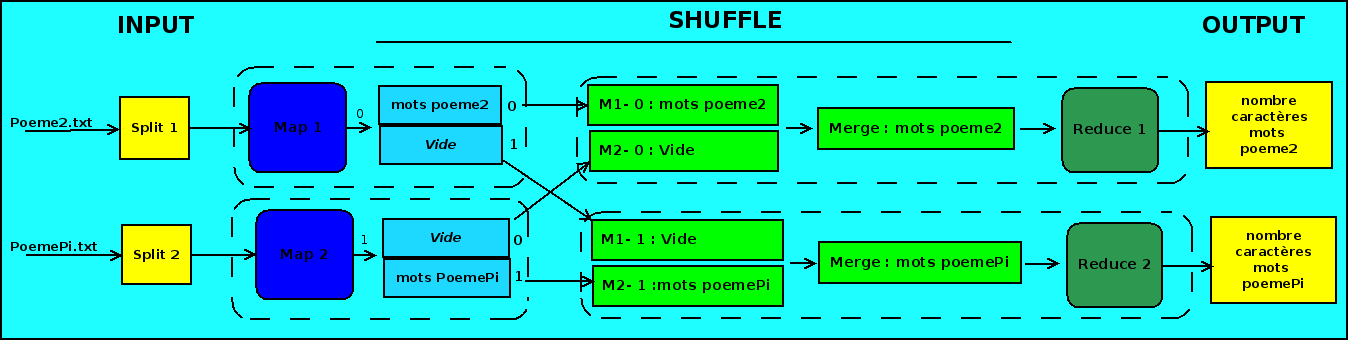
\includegraphics[angle=90, width=70mm, height=200mm]{img/diag.png}
	\caption{Graphe de communication entre les maps et les reduces}
    \end{figure}

\end{document}
